\documentclass[11pt,a4paper]{article}

\usepackage{tikz}
\usetikzlibrary{shapes}
\usepackage[utf8]{inputenc}
\usepackage{amsmath}
\usepackage{mathtools}
\usepackage{amsfonts}
\usepackage{pdfpages}
\usepackage{gauss}
\usepackage{fancyvrb}
\usepackage{hyperref}
\usepackage{graphicx}
\usepackage{url}
\usepackage{float}
\usepackage[bottom]{footmisc}

% algorithms
\usepackage{algorithm}              % algorithm float environment
\usepackage[noend]{algpseudocode}   % from algorithmicx; no "end" on functions
\newcommand*\Let[2]{\State #1 $\gets$ #2}
\algrenewcommand\algorithmicrequire{\textbf{Precondition:}}
%\algrenewcommand\alglinenumber[1]{\\footnotesize{\color{gray}#1}}

% headers and footers
\usepackage{fancyhdr, lastpage}
\pagestyle{fancy}
\fancyhf{}
\renewcommand{\headrulewidth}{0pt}
\cfoot{Page \thepage\ of \pageref{LastPage}}

% handy commands etc.
\newcommand{\eqdef}{\overset{\mathrm{def}}{=\joinrel=}}

\title{Bachelor project \\
       \vspace{2mm}
       {\LARGE Efficient DNA/RNA-sequence clustering}}
\author{Anders Kiel Hovgaard \and Nikolaj Dybdahl Rathcke}

\begin{document}
\maketitle
\thispagestyle{empty}
\newpage

\begin{abstract}
  This will eventually contain a beautiful abstract...
\end{abstract}
\thispagestyle{plain}
\pagenumbering{roman}
\newpage

\tableofcontents
\thispagestyle{plain}
\newpage

\thispagestyle{fancy}
\pagenumbering{arabic}
\section{What should be in report?}

\begin{itemize}
  \item Introduction: introducing the motivation and goals for the project.
    
  \item Terminology: clarification of USEARCH vs UCLUST, definition of
    clustering and distance metric etc.

  \item Biology: the basics about gene sequences, DNA, RNA, sequencing etc.

  \item Background: theoretical overview of the field of clustering
    \begin{itemize}
      \item Types of cluster analysis algorithms
        \begin{itemize}
          \item Hierarchical clustering (agglomerative and divisive)
          \item Graph based clustering
          \item Gready algorithm like in \texttt{UCLUST}
          \item Gready algorithm with recalculation of centroids
        \end{itemize}

      \item Distance metrics
        \begin{itemize}
          \item Edit distance (Levenshtein)
          \item d2 distance (feature based distance)
          \item Sequence alignment
        \end{itemize}

      \item Clustering "history"
    \end{itemize}

  \item Research process
    \begin{itemize}
      \item Implementing basic Levenshtein and memoized Levenshtein,
        implementing d2 distance and comparing these.
      \item Testing USEARCH 32-bit on real data
      \item Implementing very (almost naively) gready clustering algorithm.
      \item Testing clustering algorithm with d2 distance and comparing
        performance to USEARCH.
    \end{itemize}
\end{itemize}


\section{To be done}
d2 - Remembering/reading kmers somehow instead of recomputing each time?

\section{Introduction}
Clustering is the task of grouping objects so that, based on a given similarity
threshold, each object belongs to only one cluster.  This project is concerned
with the clustering of DNA and RNA sequences. Our clustering method strives to
find one centroid, a sequence that represents a cluster, that is within some
given distance of a sequence, but the centroid is not guaranteed to be the best
matching centroid.

The main motivation for this project comes from a need for efficient tools for
clustering of sequence data, and related techniques, in the microbiology
department at the University of Copenhagen. In particular, the idea for this
project comes from a collaboration between the supervisor of this project,
Rasmus Fonseca, and Martin Asser Hansen, who is a bioinformatician in the
Molecular Microbial Ecology
Group\footnote{\url{http://www2.bio.ku.dk/microbiology/}}.

Clustering huge amounts of DNA/RNA-sequences (up to 500 million strings of
500-1500 characters each) is computationally hard and there are not many
available algorithms and tools for efficient clustering of sequencing data. The
one tool \texttt{UCLUST}\footnote{\url{http://drive5.com/usearch/}} that does
the job is closed-source and considered too expensive.

This project researches the possibilities for creating an open source tool that
can match the performance of the proprietary version of \texttt{UCLUST}. We
present an implementation of a solution that uses the concept of $k$-mer
counting, for measuring the distance between sequences, and utilizes the
$k$-mers occuring in the centroids for improving the search for a centroid that
is within the given threshold distance.

\section{Terminology}
This section describes some basic terminology and notation of this text.

The words \emph{sequence} and \emph{string} will be used to denote the same
concepts, i.e. a possibly infinite, ordered list of objects, where an object
will most often be a text character.

In this text, the notion of a subsequence is different from that of a
substring: a substring $S'$ of a sequence $S$ is a consecutive, ordered list of
objects, that occurs in $S$, while a subsequence $S''$ of $S$ is a sequence
that can be obtained from $S$ by deleting some objects from the sequence
without changing the order of the objects.

% Definition of subsequence, what's a sequence, what's an alphabet, notation...

\subsection{Notation}
Let $s$ and $t$ be sequences.
\begin{itemize}
  \item $|s|$ denotes the length of $s$
  \item $s \sqsubseteq t$ denotes that $s$ is a substring of $t$
  \item $J(A,B)$ denotes the Jaccard index, or Jaccard similarity coefficient,
    of sets $A$ and $B$
\end{itemize}

\section{Background}

\subsection{Distance metrics}

\subsubsection{Edit distance}
One type of \emph{edit distance} is the \emph{Levenshtein} distance, which is a
string metric for determining the similarity between two sequences. It is
defined to be the minimum number of edits to turn the first sequence into the
other. \\
The edit operations consists of \emph{insertions}, \emph{deletions} and
\emph{substitutions}. These operations are, respectively, inserting a letter,
removing a letter and changing one letter for another. \\
The Levenshtein distance from sequence $a$ to $b$ with indicator function 
$1_(a_i\neq b_j)$, which is only $0$ when $a_i=b_j$, can mathematically be 
defined as
\begin{equation}
	\operatorname{lev}_{a,b}(i,j)= 
	\begin{cases}
	  	\max(i,j) & \text{ if} \min(i,j)=0, \\
  	  	\min \begin{cases}
        		\operatorname{lev}_{a,b}(i-1,j) + 1 \\
          	\operatorname{lev}_{a,b}(i,j-1) + 1 \\
          	\operatorname{lev}_{a,b}(i-1,j-1) + 1_{(a_i \neq b_j)}
       \end{cases} & \text{ otherwise.}
	\end{cases}
\end{equation}
where $(i,j)=(|a|,|b|)$.\\
For example, the two sequences
\begin{center}
\texttt{ACGT} \\
\texttt{ACGGC}
\end{center}
would have a distance of 2 (substituting T for G and inserting a C). \\
However, there are some cases where the relevance of the distance is arguable.
Consider the sequences
\begin{center}
\texttt{AACC} \\
\texttt{CCAA}
\end{center}
with a distance of 4. The two sequences actually have the maximal distance
possible even though they have a close resemblance to each other.


\subsubsection{Feature based distance}
A $k$-mer, or $k$-gram or simply a \emph{word}, is a sequence of length
$k \geq 0$ over some alphabet $\mathcal{A}$ of a sequence. $k$-mers are a type
of sequence \emph{feature}. An interesting feature of a sequence is the
$k$-mers that occur in that sequence.

$d2$ is a feature based distance metric, using $k$-mers as the feature. The
distance is calculated by counting the $k$-mers occurring in two sequences,
representing these occurrences as two vectors and finally taking the Euclidean
distance between these two vectors.

Let $c_x(w)$ be the number of times that a $k$-mer $w$ occurs in the sequence
$x$. Then the $d2$ distance can be defined as follows:
\begin{equation}
  d2_k(x,y) \eqdef \sqrt{\sum_{|w|=k} (c_x(w) - c_y(w))^2}
\end{equation}

As an example, the two $2$-mer frequency vectors of the sequences
\begin{align*}
  S_1 &= AGACTG \\
  S_2 &= ACAGAT
\end{align*}
over the alphabet $\mathcal{A} = \{A,C,T,G\}$, can be illustrated as follows:

\begin{table}[!h]
\centering
\scalebox{0.7}{
\begin{tabular}{c | c c c c c c c c c c c c c c c c}
        & AA & AC & AG & AT & CA & CC & CG & CT & GA & GC & GG & GT & TA & TC & TG & TT \\
  \hline
  $S_1$ &    &  1 &  1 &    &    &    &    &  1 &  1 &    &    &    &    &    &  1 &    \\
  \hline
  $S_1$ &    &  1 &  1 &  1 &  1 &    &    &    &  1 &    &    &    &    &    &    &    \\
\end{tabular}}
\end{table}

The Euclidean distance would then be calculated as
\begin{align*}
  d2_2(S_1, S_2)
    &= \sqrt{(1-1)^2 + (1-1)^2 + (-1)^2 + (-1)^2 + (1)^2 + (1-1)^2 + (1)^2} \\
    &= 2
\end{align*}

To better support distance between two sequences of different length, but
similar subsequences, the concept of a \emph{window} can be used to split the
distance calculation into comparison of substrings of length of the window
and then use the window with the least distance as the resulting distance. In
this way two sequences, where one is a prefix or postfix of the other, will
have zero distance.




\subsubsection{Sequence alignment}
\emph{Sequence alignment} is used in bioinformatics to identify regions of
similarity by arranging two or more sequences in a certain manner. Besides
shifting a sequence to a side, gaps can be inserted between objects as well. We
represent the gap with '-' and it indicates a insertion in the sequence or a
deletion from another sequence.\\
We call a column that includes - for an indel. If it does not and all object in
the column are same, then we have a match. Otherwise, it is a mismatch.\\
\begin{figure}[h!]
  \centering
  	  \begin{align*}
  	  	\mbox{\texttt{ATGCAACGA}} \\
      	\mbox{\texttt{-TGCG-CGA}}
  	  \end{align*}
  \caption{Sequence alignment of 'ATGCAACGA' and 'TGCGCGA'}
  \label{fig:seqAlignment}
\end{figure}
Figure \ref{fig:seqAlignment} displays an alignment of two sequences. In
column 1 is an indel, in column 2 are matches and in column 5 is a mismatch. 
The amount of each type can then be used in a formula to calculate the 
similarity between the sequences. Note that more than two sequences can be 
aligned in a \emph{multiple
sequence alignment}. \\
There are many alignments. Among those is an optimal alignment which is the one that is searched for. \\
\\
Both \texttt{VSEARCH} and \texttt{UCLUST} uses some kind of sequence alignment. \texttt{VSEARCH} uses a parallelized version of the dynamic programming algorithm Needleman-Wunsch, while \texttt{UCLUST} uses an heuristic procedure by default, but can be modified to use Needleman-Wunsch or Smith-Waterson. However, this will make \texttt{UCLUST} much slower.

\subsection{Cluster analysis algorithms}

\subsubsection{Hierarchical clustering}
There are typically two types of hierarchical algorithms, both of which are 
merge based, the agglomerative that works in a bottom-up manner and the 
divisive that has a top-down approach, but we focus on explaining the 
agglomerative. The agglomerative works in a bottom-
up manner where all sequences start as leaves and they are then merged 
together in clusters if they are within a given threshold.\\
\\% TODO: MAKE ILLUSTRATION
This adresses the question of what is required for a cluster to be within a 
given threshold. Besides measuring similarity between sequences with a 
distance metric, a definition for when a sequence is part of a cluster is 
needed. \\

With the \textit{single-linkage} approach, only one sequence from both 
clusters are required to be within the threshold.

In the \textit{complete-linkage} approach, all sequences from one cluster 
must be within the threshold of all sequences from the other.

In the \textit{average-linkage}, the average distance of all pairs of 
sequences is required to be within the threshold.\\
\\
The singly-linkage approach is often used in sequence clustering though it has its disadvantages as argued in \cite[pp. 62-63]{dong}

\subsubsection{Graph based clustering}


\subsubsection{Greedy algorithm like in \texttt{UCLUST}} 
The \texttt{UCLUST} algorithm is greedy and is developed so that all member
sequence have similarity $\geq$ $T$ to their centroid.  It works by processing
one sequence at a time and comparing these to the existing centroids. If a
match is found, the sequence is assigned to the matching centroid, otherwise it
becomes a centroid of a new cluster.

It is designed to also support that each centroid has a similarity $<T$ to all
other centroids, but this is not guaranteed to hold. The reason is that the
algorithm only compares a sequence to a prespecified number of centroids given
by the \texttt{-maxrejects} parameter.

It uses the $k$-mer counts to locate centroid candidates for a match, though
how it does it is not very well described.

The similarity calculations are performed with global sequence alignments as
\cite{usearch} claims that using the word counts to calculate identity is not
sensitive enough.

%TODO? \subsubsection{Greedy algorithm with recalculation of centroids}

\section{Research process}
\subsection{Starting out: Levenshtein with dynamic programming}
For a start, a naive version of the Levenshtein distance metric was
implemented, but as expected, this is absolutely useless in any practical
setting, since it does not reuse already calculated results. Therefore, this
was quickly transformed into a dynamic programming solution, which solves
subproblems just once, stores and reuses the intermediate results. This dynamic
programming bottom up solution was however still very slow, yielding a
performance of around 70 comparisons per second.

\subsection{Simple $d2$ distance}
After learning that the basic Levenshtein algorithm is far too slow for the
problem domain of this project, we turned our attention to the $d2$ distance
metric. The first version of the $d2$ distance metric algorithm is shown in
figure \ref{alg:d2_naive}. This algorithm maintains a single frequency vector,
as a map structure to allow for large $k$ which results in a large number of
possible different $k$-mers. The map is indexed using the lexicographical
position of the $k$-mer. When iterating through the first sequence, $k$-mer
counts are incremented and when iterating through the second sequence, they are
decremented. Finally all the frequencies are squared and the square root of the
sum is returned, corresponding to the Euclidean distance between frequency
vectors for the two sequences.

\begin{algorithm}
  \caption{Naive \textsc{d2} distance metric}
  \label{alg:d2_naive}
  \begin{algorithmic}[1]
    \Require{$s$ and $t$ are DNA or RNA sequences and $k \in \mathbb{Z}^+$}
    \Statex
    \Function{d2}{$s, t, k$}
      \State initialize \texttt{freq\_map}
      \For{$i \gets 0$ to $length(s) - k$}
        \State freq\_map[index\_of\_kmer(s.substring(i, k)]\texttt{++}
      \EndFor
      \For{$i \gets 0$ to $length(t) - k$}
        \State freq\_map[index\_of\_kmer(t.substring(i, k)]\texttt{--}
      \EndFor
      \State $total \gets 0$
      \ForAll{$e \in$ freq\_map}
        \State $total \gets e.value^2$  \Comment{calculate the Euclidean distance}
      \EndFor
      \State \Return $\sqrt{total}$
    \EndFunction
  \end{algorithmic}
\end{algorithm}


\subsection{$d2$ distance with windows and Jaccard index}
The current version of the $d2$ distance function uses the concept of a
\emph{window}, of a certain length, that iterates over the sequences and
calculates distances between the substrings in each window. This calculation is
done using a kind of forward differences method for reducing the calculations
to a few fixed operations for calculating the distance in the next window from
the distance in the current window. This concept is described in
\cite{hazelhurst}.

The algorithm presented here uses a window size equal to the length of the
shortest of the two sequences. Let $|s|$ be the length of the shortest of the
two sequences. To begin with the, the $k$-mers in the first $|s|$ characters of
each sequence are counted and the \emph{Manhattan} distance between these two
frequency vectors is calculated.

The Manhattan distance is simply the Euclidean distance where squaring is
replaced with absolute value and the square root is omitted, i.e. for
$u, v \in \mathbb{F}^n$, 
\begin{equation}
  d_{Manhattan} \eqdef \sum_{i=1}^{n} |u_i - v_i| \;.
\end{equation}

This distance is the distance between the subsequences in the first position of
the window. To calculate the distance in the following window, i.e. advancing
the window through the longer of the two sequences by one character, it is
decided which $k$-mers exit and enter the window, respectively, and then by
looking at whether the existing $k$-mer count in the frequency vector is
negative or positive, it can be decided whether the distance increases or
decreased by 2 or whether it stays the same. Subsequently, the frequency vector
is updated to reflect the change in the new window. The following illustrates
the idea of a window and $k$-mers exiting and entering the window:
\begin{verbatim}
      |---- window ----------|
      ACTGATCGTAGCTAGCTAGTGTTG
      ACGTAGATCGTGGATGGCTGATCGTAGCTAAGCTTAGCTGATCG.....
      ^^^^                 ^^^^
      k-mer exiting        k-mer entering
\end{verbatim}

Since the Manhattan distance can be hard to use in practice, since it is very
dependent on the length of the shortest sequence (the length of the window),
the concept of the \emph{Jaccard index}, or the \emph{Jaccard similarity
coefficient}, is used to ``normalize'' the distance to a value in the interval
$[0,1]$.

The Jaccard index of two sets $A$ and $B$ is defined as follows:
\begin{equation}
  J(A, B) \eqdef \frac{|A \cup B| - |A \cap B|}{|A \cup B|}
\end{equation}
 % TODO:  maybe actually Jaccard distance; maybe add citation

In the context of $k$-mer frequencies, the union can be interpreted as the
total number of $k$-mers in the window in the two sequences, and the
intersection as the Manhattan distance in the window.

\subsection{Evaluating distance metric}
To evaluate our implementation of the $k$-mer distance using windows and
Jaccard index, we decided to use the Levenshtein distance as reference.\\ Since
Levenshtein distance does not produce values between $0$ and $1$, we have
normalized it so it uses Jaccard index.

In figure \ref{fig:Levenshtein_vs_Kmer} is three scatter plots with the
Levenshtein distance on the $y$-axis and our version of the $k$-mer distance on
the $x$-axis. The three plots are with $k=4,k=6$ and $k=8$.

The scatter plots gives an indication about when and how sensitive our
implemented distance metric is. We want the distance to be as close as possible
to a linear function without too much variance, but not necessarily to the line
$y=x$. If it can be expressed linearly it means there is a correlation between
the two. If it can be expressed as $y=x$ (or close) it means that they measure
the same distance which is favourable.

When $k=4$ there is a linear relation when the identity $I>0.9$, but when
$I<0.9$ there is too much variance in the points from any linear function.

With $k=6$ there seems to be a linear relation when $I>0.8$. When $I<0.8$ there
is more variance though less than when $k=4$.

When $k=8$, it is very similar to $k=6$. It seems there is a linear relation
for $I>0.8$ again and when $I<0.8$ the variance is greater.

\begin{figure}
        \begin{subfigure}[b]{0.5\textwidth}
        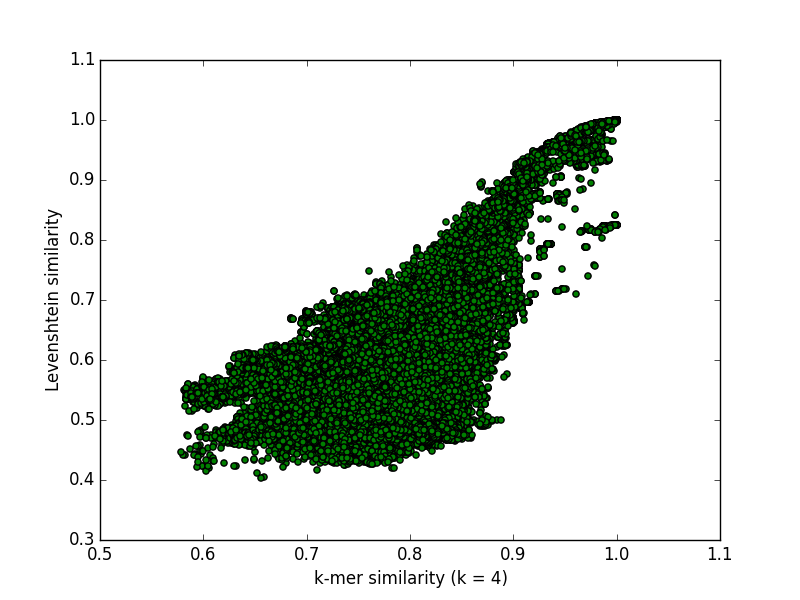
\includegraphics[scale=0.34]{graphics/k4.png}
        \end{subfigure}
        \begin{subfigure}[b]{0.5\textwidth}
        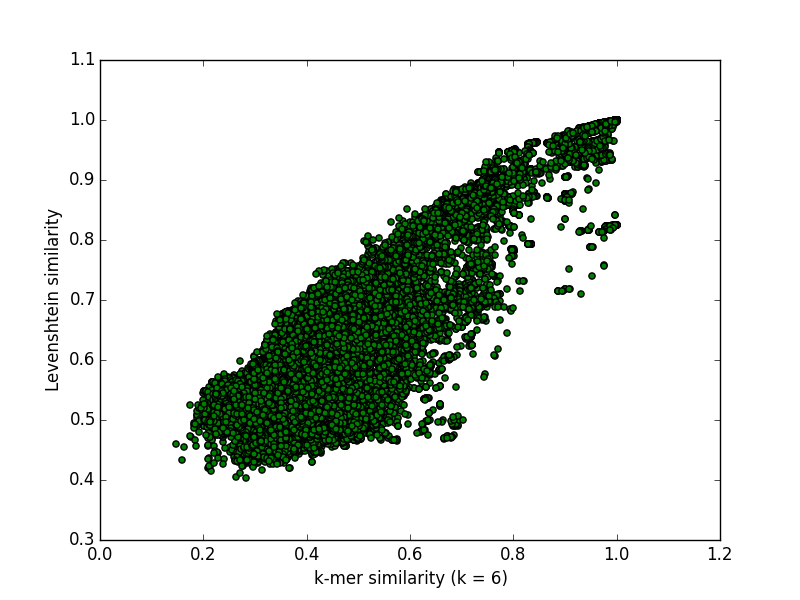
\includegraphics[scale=0.34]{graphics/k6.png}
        \end{subfigure}

  \centering
        \begin{subfigure}[b]{0.5\textwidth}
        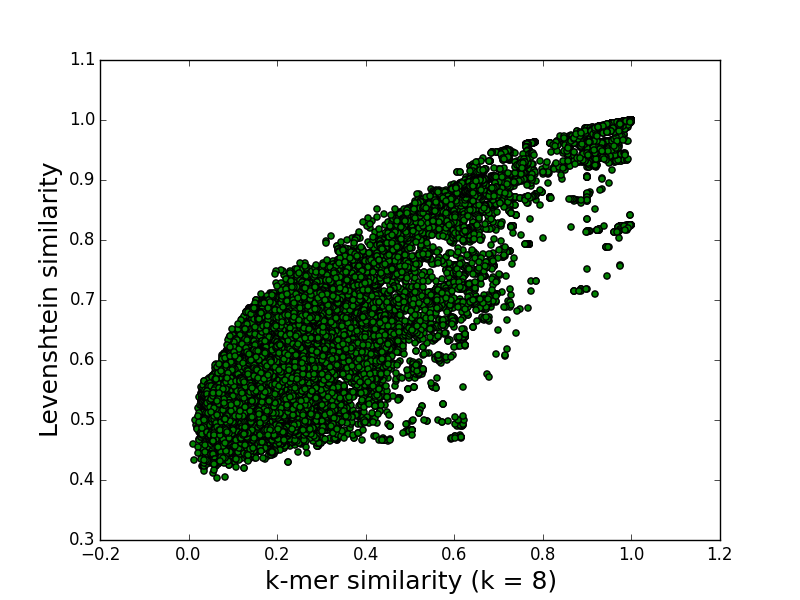
\includegraphics[scale=0.34]{graphics/k8.png}
        \end{subfigure}
\caption{Comparison of Levenshtein distance and our implementation of the
$k$-mer distance using windows and Jaccard index.}
\label{fig:Levenshtein_vs_Kmer}
\end{figure}


\subsection{``Naively greedy'' clustering algorithm} % TODO
% \item Implementing very (almost naively) greedy clustering algorithm.
Description and evaluation of a ``naively greedy'' clustering algorithm which
compares every sequence to every centroid, found so far, until a match is found
and if not, the sequence becomes a new centroid.


\subsection{\textsc{Simple\_Clust} algorithm}
We have developed a clustering algorithm, named \textsc{Simple\_Clust}
(Algorithm \ref{alg:simple_clust}), which will be described in this section.
\textsc{Simple\_Clust} works by iterating sequentially through the sequences to
be clustered; the $max\_reject$ most frequent $k$-mers for the query sequence
are calculated and for each of these most frequent $k$-mers, a centroid which
has that $k$-mer as the most frequently occurring one (if one such centroid
exists) is compared with the query sequence to check if distance is within the
given threshold. The query sequence is assigned to the cluster for the first
centroid that matches the query sequence; if no such centroid is found, out of
the maximum possible $max\_reject$ number of tries, the query sequence becomes
a centroid for a new cluster, the most frequent $k$-mer is decided and the
sequence, along with this information, is added to the collection of centroids.

This is repeated for all sequences in the input file.

\begin{algorithm}
  \caption{\textsc{Simple\_Clust}}
  \label{alg:d2_naive}
  \begin{algorithmic}[1]
    \Require{$S$ is an array of [DR]NA sequences, $k \in \mathbb{Z}^+$ and
             $max\_rejects \in \mathbb{Z}^+$, $id \in [0,1]$}
    \Statex
    \Function{Simple\_Clust}{$S, k, max\_rejects$}
      \State $cluster\_count \gets 0$
      \State $centroids \gets []$ \Comment{map from $k$-mer to sequence}
      \ForAll{$s \in S$}
        \State $mfk \gets$ $max\_rejects$ most frequent $k$-mers in $s$
        \ForAll{$m \in mfk$}
          \If{$centroids[m]$ does not exists}
            \State continue
          \ElsIf{$distance(s, centroids[m]) \geq id$}
            \State add $s$ to cluster with centroid $centroids[m]$
            \State write cluster output file
            \State break
          \EndIf
        \EndFor
        \If{matching centroid was not found}
          \State centroids.insert(mfk[0], s)
          \State write centroids output file
        \EndIf
      \EndFor
      \State \Return $cluster\_count$
    \EndFunction
  \end{algorithmic}
  \label{alg:simple_clust}
\end{algorithm}


\subsection{Comparing with UCLUST on real data}
% Testing USEARCH 32-bit on real data
% Testing clustering algorithm with d2 distance and comparing performance to
% USEARCH.
Comparing perfomance and results of the developed clustering algorithms versus
UCLUST on real data (RDP, SILVA, Amplicon etc.).

Possibly things to look into: confusion matrix, Rand index, normalized
mutual information (article: Comparing Clusterings - An Overview).


\subsection{Results}
\begin{figure}[H]
  \centering
  \begin{tabular}{ c | c }
    Metric                                        & Comparisons/second      \\
    \hline \hline
    Dynamic programming (bottom up) Levenshtein   & $\sim$ 70               \\
    \hline
    d2-distance with window, $k=4$                & $\sim$ 73000            \\
    \hline
    d2-distance with window, $k=6$                & $\sim$ 63000            \\
    \hline
    d2-distance with window, $k=8$                & $\sim$ 24000            \\
  \end{tabular}
  \caption{Performance of different distance metrics.}
\end{figure}

\begin{figure}[H]
  \centering
  \begin{tabular}{ p{12em} | c | c }
    Method  & Throughput/second   & \# of clusters \\
    \hline \hline
    \textsc{Simple\_Clust}, $k=4$,
    $max\_rejects=8$, $id=0.97$     & $\sim$ 11,400  & 444,654  \\
    \hline
    \textsc{Simple\_Clust}, $k=5$,
    $max\_rejects=8$, $id=0.97$     & $\sim$ 10,700  & 461,266  \\
    \hline
    \textsc{Simple\_Clust}, $k=6$,
    $max\_rejects=8$, $id=0.97$     & $\sim$ 9,575   & 470,516  \\
    \hline
    \textsc{Simple\_Clust}, $k=7$,
    $max\_rejects=8$, $id=0.97$     & $\sim$ 6,350   & 474,463  \\
    \hline
    \textsc{Simple\_Clust}, $k=8$,
    $max\_rejects=8$, $id=0.97$     & $\sim$ 2,750   & 475,465  \\
  \end{tabular}
  \caption{Performance of different clustering methods. Sequence data:
           \texttt{RDP\_Pro\_Full\_sort.fna}. Count: 500,000. Throughput
           specifies the number of sequences clustered per second (including
           results output to file), but excludes reading the input file.}
\end{figure}


\newpage
\begin{thebibliography}{9}
  \bibitem[Hazelhurst2003]{hazelhurst2003}
    Scott Hazelhurst,
    \emph{An implementation of the $d^2$ distance function for DNA
      sequences: The wcd $d^2$ EST clustering algorithm},
      September 2003,
      \url{http://citeseerx.ist.psu.edu/viewdoc/download?doi=10.1.1.9.4289&rep=rep1&type=pdf}.

    \bibitem[Dong2007]{dong2007}
      Guozhu Dong, Jian Pei, \emph{Sequence Data Mining},
      Springer, 2007.
\end{thebibliography}

\end{document}
